\documentclass{article}

\usepackage{verbatim}
\usepackage{amsmath}

\author{Paul Kröger \and Ali Bektas}
\title{Symbolic Music Similarity and Music Plagiarism}


\usepackage{graphicx}
\graphicspath{ {../images/} }

\begin{comment}
	Bitte zuerst hier lesen!

		Während du das Outline liest , wirst du Zitate sehen die z.b so aussehen : one_point_one
		Diese sind ihre Adressen im Directory Tree. Ich habe dementsprechenden Ordner erstellt die Namen wie 1/ , 1/1.2/1.23
		haben. In jedem Ordner muss (wichtig!) einen bib.txt File geben , in dem es die Bibliographie in MLA und BibTex Formatten geben. 
		Bitte mach Zitate dementsprechend ( 1/1.2/1.2.3 also 1.2.3 wäre z.B \cite{one_point_two_point_three}).

	\cite{lost} bedeutet : Es kam irgendwo ran , aber wo weiß ich nicht mehr.
	Du kannst auch solche merkwürdige Namen nutzen aber dann bitte schreib hier was diese bedeuten.

\end{comment}


\begin{document}
	\maketitle

	\section*{Abstract} 

	As it becomes ever more easy to produce music from one's own home, the challenge of detecting plagiarized 
	parts becomes more important. Detection of such plagiarism through subjective reasoning is a time consuming 
	effort and must inevitably be replaced by automatized solutions.The problem of detecting such plagiarisms 
	is strongly connected to determining similarity between two pieces by means of music similarity approaches. 
	Thus , the detection of plagiarized works is based on techniques of music similarity. Not every 
	approach in music similarity is however useful , since music similarity is a broader term than fetching 
	related songs based on their melody , rhythm and so on. 
	Due to melodic similarity being the crucial factor in plagiarism cases \cite{one_point_one}
	\begin{comment}
	See 1.1 page 188
	______________________
	Although plaintiffs invariably claim musical rather than melodic infringement, courts pay little attention 
	to rhythm, harmony, or other elements of music.
	\end{comment}
	, and rightly so since the 
	melody is according to \cite{lost} the most important aspect in a song for the human ear,
	\begin{comment}
		Here a resource about psychoacoustics.
	\end{comment}
	we will focus on melodic similarity detection . The main emphasis of this paper is therefore to 
	explore the ways in deciding whether two pieces are similar, what metrics can be used to do so and how 
	appropriate the different approaches are.  
	
	\section*{Outline}


	\section*{Introduction}
		Plagiarism detection algorithms differ from music similarity algorithms in that they answer a Yes/No question whereas music similarity algorithms return a list of best results.

	\begin{comment}
	See 1.1 page 188
	______________________

		The author himself took (1) from :
			Northern Music Corp. v. King Record Distribution Co., 105 F. Supp. 393 (S.D.N.Y. 1952)
		1) The pronouncements in Northern Music v. King Record are typical : rhytmic originality is nearly impossible to achieve , harmony is simply the application of well-known rules , and neither can be the subject of copyright.
		
		and 2 from:
			Jollie v. Jacques, 13 F. Cas. 910 (C.C.S.D.N.Y. 1850)

		2) For federal courts at least , the originality the sine qua non of copright in music lies in melody. The melody "requires genius for its construction"(Jollie v. Jacques 1850 , 913). It is the "fingerprint of a musical work and "a mere mechanic can make the adaptation or accompaniment".

	\end{comment}
	

	\section{Approaches for symbolic data}
		Symbolic data in music are representations of a musical structure usually based on pitch related and temporal informations. Modern western techniques date back to ...

		In modern digitalized techniques used in representing a musical piece there are more than the two abovementioned dimensions. 

		Rhytmical structure is as important since depending on the rhythm  , notes become more significant within a piece.
		

		\begin{figure}[h!]
			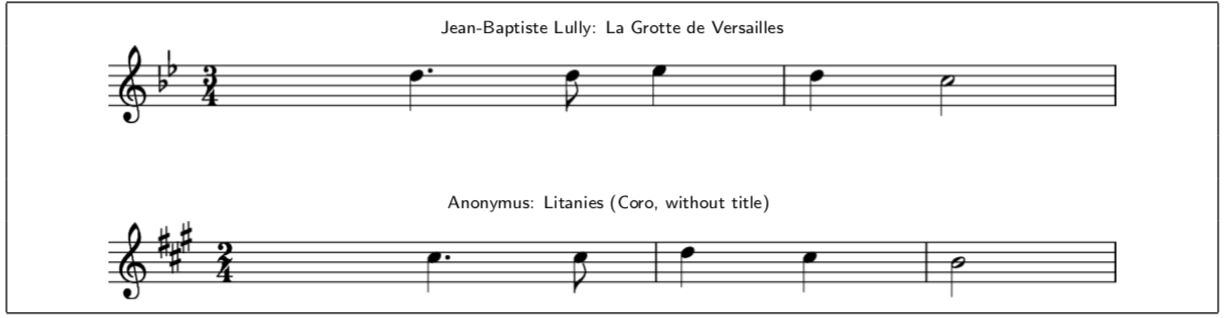
\includegraphics[width=\textwidth,height=\textheight,keepaspectratio]{figure_1_of_3}
			\caption{Even though the notes are the same they are heard different since rhythm changes how a melodic sequence is percieved.}
 		\end{figure}

		\subsection{Symbolic Music Similarity}
			\begin{comment}

			Given two or more sequences of notes, symbolic melodic similarity (SMS) 
			aims to evaluate their degree of likeness, as human listeners are able
			to do. \cite{two}
			\end{comment}
			The MIREX (Music Information Retrieval Exchange) is a community who arranges contest in different topics of Music Information Retrieval. Since 2005 there has been a number of algorithms which have suggested new approaches in the field.
			\cite{two} places these algorithms with into three categories:
				The ones that use \label{categories}
				\begin{enumerate}
					\item Mathematics
					\item Cognition
					\item Music Theory
				\end{enumerate}

			\subsubsection{Algorithms of Category 1}
				The algorithm proposed by \cite{one} aims to convert melodies into "orthagonal polygonal chains" and then "find the minimum area of 
				minimum area between two lines and two horizontal edges".

 
 				\begin{figure}[h!]
					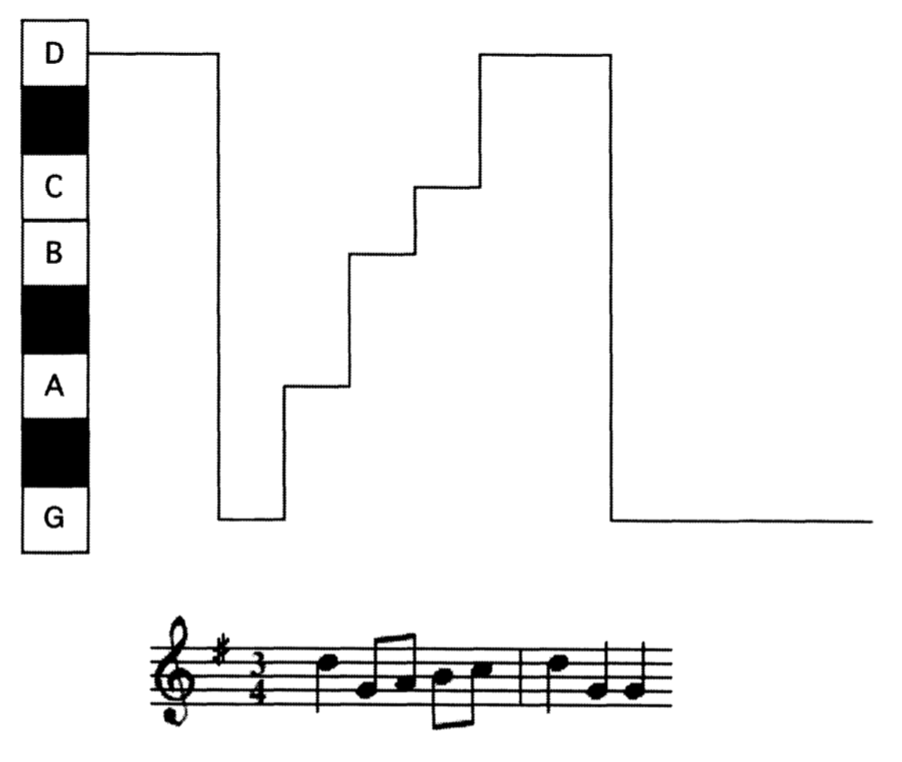
\includegraphics[width=\textwidth,height=\textheight,keepaspectratio]{figure_1_of_1}
					\caption{Source: \cite{one}}
				\end{figure}

			\vspace{200px}
			\subsubsection{Algorithms of Category 2}
					An algorithm proposed by \cite{two_point_five} uses the Implication/Realization Model (IMR).
					We will discuss IMR.

					A MIDI-formatted input undergoes Melody Seperator , which as the name suggests turns melody into segments.
					This paper emphasizes that the intervalic information between two notes must be further detailed by the direction of pitch change.


					This algorithms incorporates n-gram method.
					What is n-gram method?

					Similarity is finally calculated by

					\begin{equation}
						S(query , comparison) = \frac{n}{max(a,b)}
					\end{equation}
					{Where a and b are reprectively element count of query melody and melody compared.}


					

			\newpage
			\subsubsection{Hybrid Algorithms}
				Hybrid algorithms are the algorithms , that it incorporate all of the abovementioned (See \ref{categories}) categories. This is done by taking a linear combination of several single algorithms.
 
				The SIMILE \cite{two_point_two}:
					The algorithms that are used 
						\begin{itemize}
							\item Edit Distance: e.g. Mongeau \& Sankoff, (1990)
							\item n-grams: e.g. Downie (1999)
							\item Geometric distance: Steinbeck (1982);O'Maidin (1998)
							\item Correlation coefficient: e.g. Steinbeck, (1982)
						\end{itemize}

					\begin{align*}
						optP = 0.31 \cdot joint412 &+ 1.37 \cdot rawEd \cdot connEd (1) + 0.643 \cdot rawEd \cdot harmCoEA\\
						&– 1.55\cdot connEd \cdot bGrCoorF\\
						&+ 0.65\cdot bGrCoorF\cdot rhytFuzz\\
						&– 0.39\cdot harmCoEA\cdot rhytFuzz – 0.133	
					\end{align*}

					We will explain what these are.




	\section{Approaches for plagiarism detection}
	
        Here we will introduce different approaches to automatically detecting plagiarisms in music.
	
        \subsection{Fuzzy vectorial-based similarity detection}
            An algorithm proposed by \cite{five} that constructs a vectorial representation of a melody consisting of its intervalic changes and the corresponding rhythm. These representations are then used to calculate a fuzzy number to determine similarity between melodies. 
            Vectorial melodic distance between two subvectors of length k  is then calculated by the following formula : 
            \begin{equation}
                D(s1,s2)=(D_m(s1,s2),D_r(s1,s2))
            \end{equation}
            where
            \begin{equation}
             D_m(s1,s2) = \sqrt{\sum_{i=1}^k |n_i * V_{M_1} * getPos(n_i) - m_i * V_{M_2} * getPos(m_i)|^2}
            \end{equation}
            and
            \begin{equation}
               D_r(s1,s2) = \sqrt{\sum_{i=1}^k |d_i * R_{M_1} * getPos(d_i) - t_i * R_{M_2} * getPos(t_i)|^2}
            \end{equation}
            
            The vectorial melodic distance is the used to calculate a Fuzzy Number. We will explain how this process works.



            
        
        
			

	\section*{Conclusion}

		In this paper we have reviewed various algorithms for measuring symbolic melodic similarity and algorithms for detecting music plagiarism...

		A pair of sentences about why plagiarism being a Yes/No question makes trouble since general algorithms in music similarity are not yet well established to be able to provide a unified solution to music of all genres.


	\begin{thebibliography}{9}
		\bibitem[1]{one}
		G.Aloupis,T.Fevens,S.Langerman,T.Matsui,A.Mesa, Y. Nufiez, D. Rappaport, G. Toussaint. Computer Music Journal , 30:3, pp. 67-76, Fall 2006.
		\bibitem[2]{one_point_one}
		Cronin, C. 1998. "Concepts of Melodic Similarity in
		Music-Copyright Infringement Suits."InW.B.Hewlett and E. Selfridge-Field,eds. Melodic Similarity: Concepts, Procedures,and Applications. Cambridge, Massachusetts:MITPress,pp. 187-209.
		\bibitem[3]{two}
		Symbolic Melodic Similarity: State of the Art and Future Challenges
		Valerio Velardo,Mauro Vallati and Steven Jan
		Computer Music Journal, 40:2, pp. 70–83, Summer 2016 doi:10.1162/COMJ a 00359
		2016 Massachusetts Institute of Technology.
		\bibitem[4]{two_point_two}
		Velardo, Valerio, Mauro Vallati, Steven Jan.
		"Symbolic melodic similarity: State of the art and future challenges." Computer Music Journal 40.2 (2016): 70-83.
		\bibitem[5]{two_point_five}
		Sakurako Yazawa, Yuhei Hasegawa, Kohei Kanamori and Masatoshi Hamanaka
		Melodic Similarity based on Extension Implication-Realization Model
		Music Information Retrieval Exchange , 2013.
		\bibitem[6]{five}
		R. D. Prisco, D. Malandrino, G. Zaccagnino, and R. Zaccagnino, “Fuzzy
        vectorial-based similarity detection of music plagiarism,” in 2017 IEEE
        International Conference on Fuzzy Systems, FUZZ-IEEE 2017, Naples,
        Italy, July 9-12, 2017, 2017, pp. 1–6.


	\end{thebibliography}

\end{document}
